\section{INTEGRATION} \label{sec:integration}
We defined an interface named \texttt{ObjectRecogniser} to facilitate multiple implementation of object recognizer. The image recognition framework was developed for the \texttt{ObjectRecogniser} contract. The main part of this contract is a function that accepts image data and returns list of \texttt{RecognisedObject}s

%% TODO: Summarize the challenges
%% TODO: List the available methods
The following methods of integration were investigated in the order of listing:
\begin{itemize}
\item Command Line Invocation
\item Java Native Interface
\item gRPC Remote Procedure Calls
\item Representational State Transfer API
\end{itemize}

\begin{figure*}
	\includegraphics[width=\textwidth,height=5cm]{tensorflow-tika-integration}
	\caption{Tika and Tensorflow Integration}
	\label{fig:tf-tika-integration}
\end{figure*}

%% 1. CLI
\subsection{Command Line Invocation (CLI)} \label{sec:int-cli}
Command Line Invocation is the most simple way of integration. We created a python based CLI tool as an entry point to tensorflow's image recognition network. This tool inspected the environment for its requirements. When its requirements were not met it simply failed by reporting the failure. 
Apache Tika executed in the JVM process where as on every invocation of CLI tool, a new native process was created and destroyed. Tika passed image path as command line argument to the tool as shown in Figure \ref{fig:tf-tika-integration} (a). The tool parsed the arguments, then passed the content to tensorflow network and reported the results by printing it to standard output. Tika parser then read the result from its output stream. The pros and cons are described in the Section \ref{sec:eval-cli}
%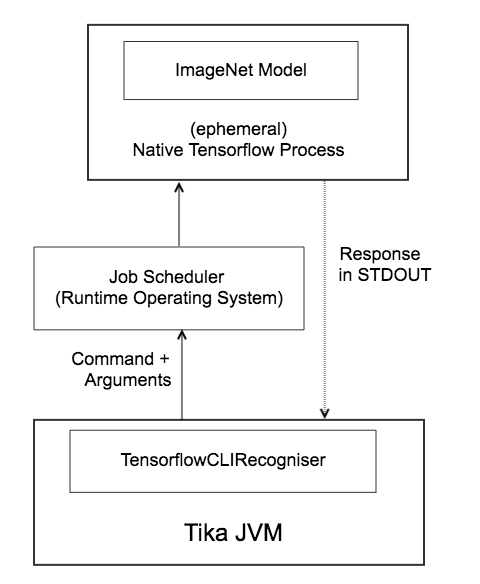
\includegraphics[scale=0.40]{tika-tflow-cli-design}

%% 2. JNI
\subsection{Java Native Interface (JNI)} \label{sec:int-jni}
The next approach we investigated was the Java Native Interface (JNI). JNI is the vendors' recommended way of integrating native code libraries to Java frameworks\cite{}. JNI acts as glue between bytecode instructions that runs within Java Virtual Machine (JVM) and the native  code instructions that runs directly on the CPU. Theoretically, this is the best way of merging JVM world with the native code\cite{}. At runtime, the bytecode of Tika (caller) and native code of tensorflow (callee) runs within the single process from the operating system's perspective as shown in Figure \ref{fig:tf-tika-integration} (b).

%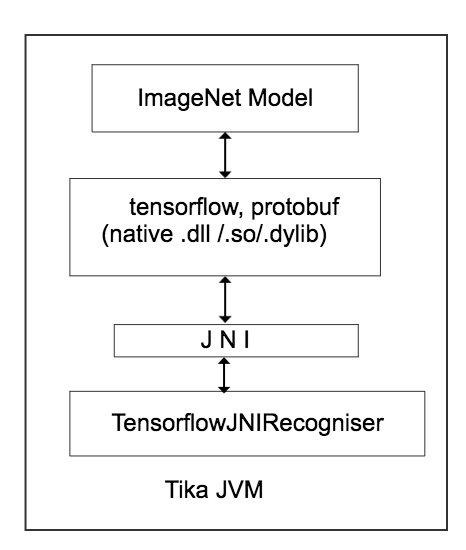
\includegraphics[scale=0.40]{tika-tflow-jni-design}

%% 3. RPC
\subsection{gRPC Remote Procedure Calls (gRPC)} \label{sec:int-rpc}
The developers of Tensorflow framework recommended to use gRPC based integration for the production systems\cite{goog-tfserve}. gRPC is a client-server based architecture in which caller acts as a RPC client and callee serves as a server in a different address space. Unlike traditional RPC frameworks, gRPC is a high performance, CPU and bandwidth efficient transport on top of HTTP/2 that supports full duplex streaming\cite{about-grpc}. In our case, we embedded gRPC client in Tika JVM and exported Tensorflow image recognition capabilities as remote procedures via gRPC service. We used Tensorflow Serving, a gRPC server implemented in C++, and also created a docker container to host it.

%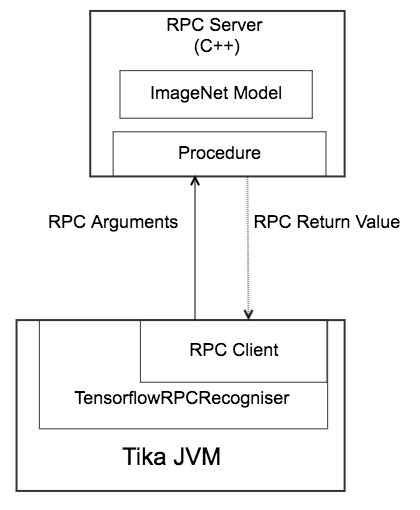
\includegraphics[scale=0.40]{tika-tflow-RPC-design}

%% 4. REST
\subsection{Representational State Transfer (REST) Application Programming Interface (API)} \label{sec:int-rest}
Representation State Transfer (REST) is a popular client-server architecture paradigm for connecting heterogeneous systems without the need of states\cite[Chapter~5]{Fielding:2000:ASD:932295}. The REST application programming interfaces (API) is powered by an HyperText Transfer Protocol (HTTP) which abstracts the complexities of Transmission Control Protocol.
We crated REST API for tensorflow image recognition using python Flask\cite{}. The Flask based HTTP service registered a TCP port and offered HTTP API end points as shown in Figure \ref{fig:tf-tika-integration} (d).
An API end point accepted HTTP POST requests with image data in the multi-part-form body. This service loaded the InceptionV3Net \cite{SzegedyVISW15} model during the initialization phase and held the model in memory for reusing it during the future HTTP Requests.

% \begin{figure}[h]
%     \centering
%     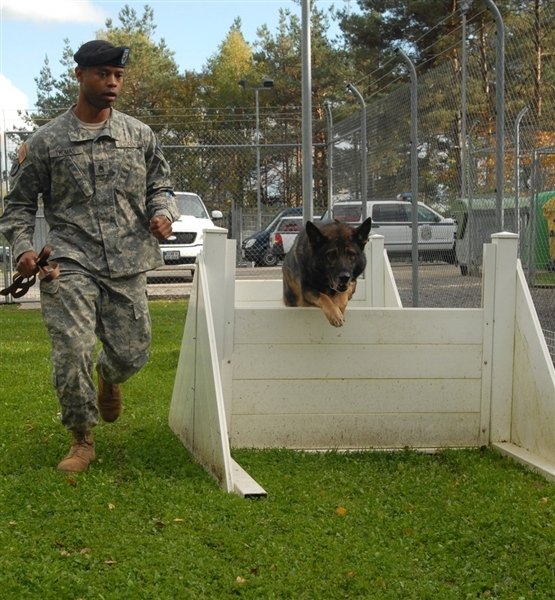
\includegraphics[width=\columnwidth]{military_dog}
%     \caption{Military Person with a German Shepherd Dog \newline Courtesy: Wikimedia Commons}
%     \label{fig:military-dog}
% \end{figure}

% The REST API, upon recognizing the objects in the image \ref{fig:military-dog}, returned the response in the JSON format with the following structure:

% \begin{lstlisting}[language=json, label=code:json-output,
% 	frame=single, xleftmargin=5.0pt, xrightmargin=5.0pt,
%     caption=JSON Response from REST API]
% {
%   "confidence": [ 0.362026, 0.130613],
%   "classnames": [
%     "German shepherd, alsatian",
%     "military uniform"
%   ],
%   "classids": [211, 866 ],
%   "time": {
%     "read": 1,
%     "units": "ms",
%     "classification": 257
%   }
% }
% \end{lstlisting}

On the other side of the system, we implemented the class \texttt{TensorflowRESTRecogniser} which used HTTP Client to communicate with REST API. This implementation of \texttt{ObjectRecogniser} converted the image data to HTTP POST request with multipart form data and sent it to REST API. It parsed the JSON response to retrieve the object names, ids and confidence scores. We also created a docker specification for bootstrapping the tensorflow image recognition REST API for semi automated deployment of the system.

%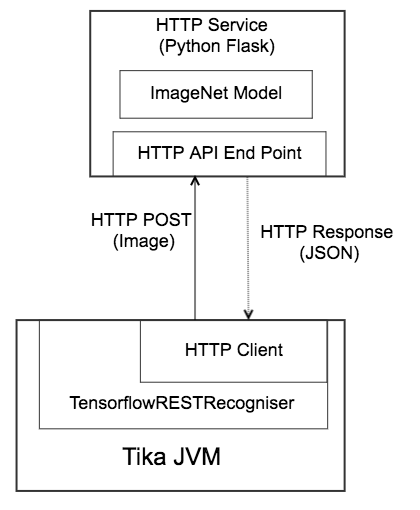
\includegraphics[scale=0.40]{tika-tflow-rest-design}
